% !TeX spellcheck = cs_CZ
%     An overview of high school mathematics
%---------------------------------------------------------------------------------------------------
% intro_LA.tex
%---------------------------------------------------------------------------------------------------
\chapter{Historie matematické analýzy}\label{mai:IchapXII}
\minitoc
  %===============================Kapitola: Determinanty===========================================
  \section{Determinanty}
    Abychom mohli nadefinovat determinant, budeme muset vědět, jak vypočítat permutaci entice, 
    respektive znaménko permutace.
    \subsection{Permutace}
      \begin{definition}\label{permutace}
        Nechť \(\mathbf{M}\) je libovolná konečná množina. Permutací množiny \(M\) nazýváme 
        zobrazení \(\pi\) množiny \(\mathbf{M}\) na sebe.
      \end{definition}
      
      \begin{example}%(Damlová  Nagy, 1985, str. 34)
        Permutace \(\pi\) množiny \(\mathbf{M}= \lbrace a,b,c,d\rbrace\) je např. zobrazení 
        \(\pi\), definované předpisem:
        \begin{equation}\label{permutace_zadani}
          \pi\left(a\right) = c, \,
          \pi\left(b\right) = d, \,
          \pi\left(c\right) = b, \,
          \pi\left(d\right) = a,
        \end{equation}
        Místo tohoto zápisu se však používá přehlednější zápis ve tvaru matice typu \((2,4)\):
        \begin{equation}\label{LA:eq_perm_exam}
            \begin{pmatrix}
            a & b & c & d \\
            c & d & b & a
            \end{pmatrix}
        \end{equation}
        kde v prvním řádku jsou vypsány všechny prvky množiny \(\mathbf{M}\) (v libovolném pořadí) 
        a ve druhém řádku je pod každým prvkem zapsán jeho obraz v permutaci. Tutéž permutaci však 
        můžeme zapsat ve tvaru matice několika různými způsoby. Například mohou být zapsány takto:
        \begin{equation}
          \begin{array}{cc}
            \begin{pmatrix}
              b & a & c & d \\
              d & c & b & a
            \end{pmatrix},         & 
            \begin{pmatrix}
              d & c & b & a \\
              a & b & d & c
            \end{pmatrix}          \\
            \begin{pmatrix}
              d & c & a & b \\
              a & b & c & d
            \end{pmatrix},         &
            \text{apod.}
          \end{array}
        \end{equation}
      \end{example}

      Zřejmě všechny čtyři uvedené zápisy permutace rov. \ref{LA:eq_perm_exam} ve tvaru matice se 
      liší navzájem pouze pořadím sloupců. Aby bylo možné zapsat každou permutaci množiny 
      \(\mathbf{M}\) ve tvaru rov. \ref{LA:eq_perm_exam} jediným způsobem, je nutné zvolit pevné 
      pořadí prvků množiny \(\mathbf{M}\)  a v zápisu permutace uvádět prvky matice \(\mathbf{M}\)  
      v prvním řádku v tomto pořadí. Avšak známe-li toto pořadí prvků množiny \(\mathbf{M}\), je 
      pak  obvykle zbytečné jej v zápisu permutace uvádět, ale stačí uvést pouze pořadí obrazů, tj. 
      druhý řádek. Zvolíme-li např. v naší množině \(\mathbf{M}\) pevné pořadí prvků \(\lbrace 
      a,b,c,d\rbrace\), pak permutaci rov. \ref{permutace_zadani} zapíšeme jako uspořádanou 
      čtveřici \(\lbrace c,d,b,a\rbrace\).
  
      \begin{definition}\label{def_permutace_ntice}
        Když vytváříme uspořádanou \(n\)-tici navzájem různých prvků \(n\)-prv\-ko\-vé množiny 
        \(\mathbf{M}\), přiřazujeme každému prvku množiny \(\mathbf{M}\) právě jedno přirozené 
        číslo, index příslušného prvku, z množiny prvních \(n\) přirozených čísel.
        \begin{equation}\label{permutace_ntice}
          \pi = \lbrace 1, 2, 3, \ldots, n\rbrace
        \end{equation}
      \end{definition}
  
      Proto každé permutaci uspořádané \(n\)-tice prvků množiny \(\mathbf{M}\) odpovídá jednoznačně 
      permutace příslušných indexů tj. permutace množiny \ref{permutace_ntice} z definice 
      \ref{def_permutace_ntice}. Stačí se tedy omezit při vyšetřování permutací n-prvkové množin 
      na vyšetřování permutací množiny \ref{permutace_ntice}. Permutace \(\pi\) množiny 
      \ref{permutace_ntice} budeme zapisovat jako uspořádané \(n\)-tice \(\left(\pi(1), \pi(2) 
      ,\ldots, \pi(n)\right)\), kde \(\pi(i)\) je číslo z množiny \ref{permutace_ntice}, které 
      permutace \(\pi\) přiřazuje číslu \(i\).

      \begin{example}\label{ex_celk_pocet_permutaci}
        \textbf{Spočítejme celkový počet permutací množiny}. V každé uspořádané \(n\)-tici může být 
        na prvním místě kterákoli z \(n\) cifer, na druhém místě kterákoli ze zbývajících \(n-1\) 
        cifer (kromě té, která je na prvním místě), na  třetím místě každá ze zbývajících \(n-2\) 
        cifer atd. Je tedy celkový počet všech permutací \(n\)-prvkové množiny \(n(n-1)(n-2)\cdot 
        \ldots \cdot2\cdot1\). Toto číslo se zapisuje pomocí symbolu \(n!\) (čti 
        \textbf{n-faktoriál}).
      \end{example}
      
      \begin{definition}\label{def_inv_perm}\textbf{Inverze v permutaci}:
        Inverzí v permutaci \(\left(i_1,i_2,…,i_n \right)\) rozumíme každý výskyt takové dvojice 
        čísel, že větší stojí před menším, tj. vlevo od něj.
      \end{definition}  
   
  %=========================== Kapitola: Vlastní čísla a vlastní vektory ==========================
  \section{Vlastní čísla a vlastní vektory}
    \subsection{Motivace} 
      \textbf{Poznámka}: Je-li \(\mathcal{A} : \mathcal{V} \rightarrow \mathcal{V}\) lineární 
      zobrazení z prostoru \(\mathcal{V}\) do prostoru \(\mathcal{V}\) (nikdy se takové zobrazení 
      nazývá lineárním operátorem), pak je přirozeným požadavkem najít takovou bázi prostoru 
      \(\mathcal{V}\), že je matice zobrazení $\mathbf{A}$ v této bázi co nejjednodušší, např. má 
      následující strukturu
      \begin{equation*}
         \mathbf{A}=
           \left(\begin{array}{ccccc}
             \boxed{A_1}       &             &       &       & 0   \\
                 & \boxed{A_2} &             &       &             \\
                 &             & \boxed{A_3} &       &             \\
                 &             &             &\ddots &             \\
              0  &             &             &       & \boxed{A_k}
            \end{array}
           \right),
     \end{equation*}
     kde \(A_k\) jsou čtvercové matice malého řádu (nejlépe \(1\) nebo \(2\)) a ostatní prvky 
     matice jsou nulové. Problém najít bázi, aby v ní matice zobrazení měla diagonální tvar (kde 
     \(A_k\) jsou skaláry), vede k pojmu vlastní číslo a vlastní vektor matice.

      \begin{definition} 
        Nechť \(\mathbf{A}\in \mathcal{C}^{n,n}\) (matice je čtvercová řádu \(n\)).
        \begin{equation}
          \mathbf{A} = (a_{ij}) =
            \begin{pmatrix}
              a_{11} & a_{12} & \ldots & a_{1n} \\
              a_{21} & a_{22} & \ldots & a_{2n} \\
              \vdots & \vdots & \ddots & \vdots \\
              a_{n1} & a_{n2} & \ldots & a_{nn}
            \end{pmatrix}
        \end{equation}

        Jestliže platí
        \begin{equation}\label{eq:vl_number}
          \mathbf{Au} = \lambda\mathbf{u}
        \end{equation}
        pro jisté komplexní číslo \(\lambda\in\mathcal{C}\)  a jistý nenulový vektor 
        \(x\in\mathcal{C}^n, \mathbf{u}\neq\Theta\), potom číslo \(\lambda\) nazýváme 
        \textbf{vlastním číslem} matice \(\mathbf{A}\) a vektor \(\mathbf{u}\) \textbf{vlastním 
        vektorem} příslušným k tomuto vlastnímu číslu. Množinu všech vlastních čísel nazýváme 
        \textbf{spektrem matice} \(\mathbf{A}\). Pokud rov. \ref{eq:vl_number} rozepíšeme, dostaneme
        \begin{equation}
          \begin{pmatrix}
            a_{11} & a_{12} & \ldots & a_{1n} \\
            a_{21} & a_{22} & \ldots & a_{2n} \\
            \vdots & \vdots & \ddots & \vdots \\
            a_{n1} & a_{n2} & \ldots & a_{nn}
          \end{pmatrix}   \cdot
          \begin{pmatrix}
            u_{1} \\  u_{2} \\ \vdots \\  u_{n} \\
          \end{pmatrix}    =\lambda\cdot
          \begin{pmatrix}
            u_{1} \\ u_{2} \\ \vdots \\ u_{n} \\
          \end{pmatrix}
        \end{equation}
        můžeme ji rovněž psát ve tvaru
        \begin{equation*}
            \begin{pmatrix}
            \setlength{\arraycolsep}{3pt}
              a_{11} -\lambda & a_{12}           & \ldots & a_{1n} \\
              a_{21}          & a_{22} -\lambda  & \ldots & a_{2n} \\
              \vdots          & \vdots           & \ddots & \vdots \\
              a_{n1}          & a_{n2}           & \ldots & a_{nn}-\lambda
            \end{pmatrix} \cdot
          \begin{pmatrix}
            u_{1} \\ u_{2} \\ \vdots \\ u_{n} \\
          \end{pmatrix}  =
          \begin{pmatrix}
              0 \\ 0 \\ \vdots \\ 0 \\
            \end{pmatrix}
        \end{equation*}
      \end{definition}

       Tato soustava rov. je \textbf{homogenní} a stručně ji můžeme zapsat
      \begin{equation}\label{vv_hom_zapis}
        \left(\mathbf{A} - \lambda\mathbf{I}\right) = \mathbf{0}
      \end{equation}
      Homogenní soustava má \emph{netriviální řešení}, právě když je determinant matice soustavy 
      roven  nule, tj. v případě soustavy rov. rov. \ref{vv_hom_zapis} platí
      \begin{equation}\label{vv_hom_reseni}
        |\mathbf{A} - \lambda\mathbf{I}| = \mathbf{0}
      \end{equation}
      Determinant \(A(\lambda)=|\mathbf{A} - \lambda \mathbf{I}|\) nazýváme 
      \textbf{charakteristický polynom} matice \(\mathbf{A}\) - jedná se o polynom stupně \(n\) v 
      proměnné \(\lambda\), který má v oboru komplexních čísel \(n\) kořenů. Rovnici 
      \(A(\lambda)=0\) nazýváme \textbf{charakteristická rovnice matice \(\mathbf{A}\)} - jejími 
      kořeny jsou \textbf{charakteristické hodnoty} (resp. \textbf{vlastní čísla}) 
      \textbf{matice} \(\mathbf{A}\).
            
      \begin{note}
        U vlastních čísel studium pouze reálných matic ztrácí smysl, protože i 
        reálná matice může mít komplexní vlastní čísla. Proto se uvažuje obecná komplexní matice.
      \end{note}
      
      \begin{note}
        Podmínka existence nenulového vektoru \(\mathbf{u} = \Theta\) v definici 
        vlastního čísla je nezbytná: kdyby bylo připuštěno i \(\mathbf{u} = \emptyset\), potom by 
        každé komplexní číslo bylo vlastním číslem a definice by ztratila smysl.
      \end{note}
      
      \begin{note}
        Odpovídá-li matice \(\mathbf{A}\) matici nějakého zobrazení \(\mathcal{A}\), pak každý 
        nenulový vektor z jádra zobrazení \(\ker\mathcal{A}\) je vlastním vektorem příslušným 
        vlastnímu číslu \(\lambda\). Je-li \(\ker\mathcal{A} = \{\Theta\}\) 
        (je-li matice \(\mathbf{A}\) regulární), pak \(\Theta\) není vlastním číslem matice 
        \(\mathbf{A}\).
      \end{note}

      %---------------------------------------------------------------
        % !TeX spellcheck = cs_CZ
\begin{mathexam}{Ortogonální projekce v prostoru \(\mathcal{R}^3\)}{exam012}
    Je-li \(\mathbf{P}\) matice ortogonální projekce v prostoru \(\mathcal{R}^3\) na nějaký 
    podprostor \(\mathcal{U}\) (\(\mathcal{U}\) je tedy buď rovina nebo přímka procházející 
    počátkem), pak pro každý vektor \(\mathbf{u}\in\mathcal{U}\) platí \(\mathbf{Pu} = 
    \mathbf{u}\), všechny vektory z \(\mathcal{U}\) (s výjimkou nulového vektoru \(\Theta\)) 
    jsou vlastními vektory matice $\mathbf{P}$ příslušné vlastnímu číslu \(\lambda\). Prostor 
    \(\mathrm{U}^\bot\) je roven jádru projekce (nulovému prostoru matice \(\mathbf{P}\)), 
    a tedy každý vektor z ortogonálního doplňku \(\mathcal{U}\) (s výjimkou \(\Theta\)) je 
    vlastním vektorem příslušným k vlastnímu číslu \(0\).

    {\centering
      \captionsetup{type=figure}
      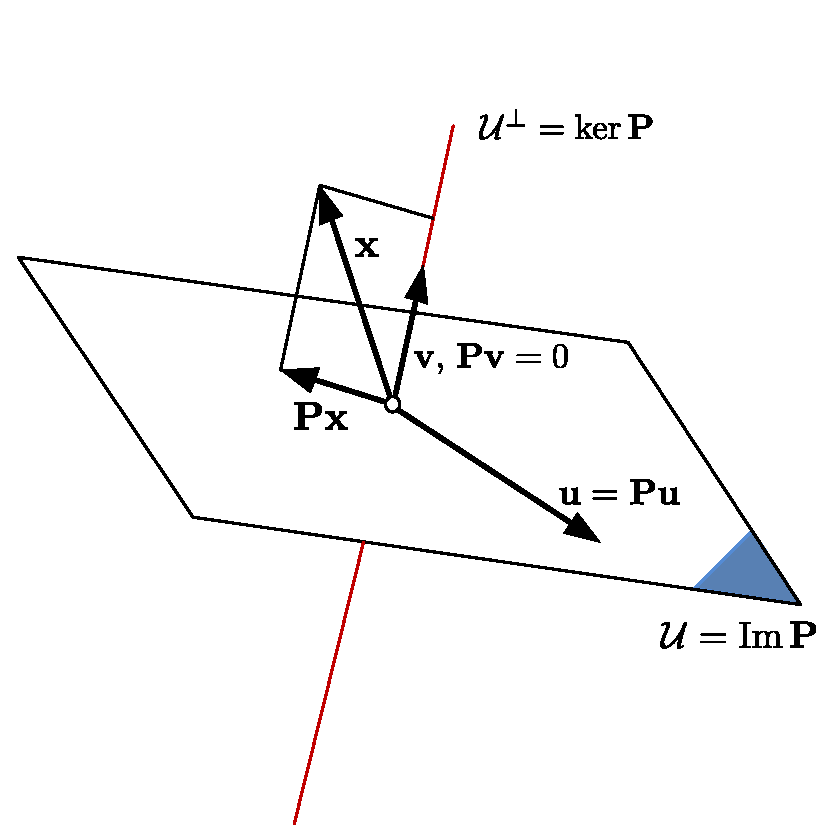
\includegraphics[width=0.5\linewidth]{mai_fig024.pdf}
      \captionof{figure}{K příkladu \ref{mai:exam012}}
      \label{mai:FIG016}
      \par}

\end{mathexam}
      %---------------------------------------------------------------

      %---------------------------------------------------------------
        % !TeX spellcheck = cs_CZ
\begin{mathexam}{Určete spektrum matice a její spektrální poloměr následující matice
  \begin{equation*}\label{pr:spektrum_matice}
    \mathbf{A} =
      \begin{pmatrix}
        2  &        2    & 0 \\
       -3  &       -3    & 5 \\
        0  & -\num{0.25} & 2
      \end{pmatrix}
  \end{equation*}
  }{exam013} 
  \textbf{Řešení}: Spektrum matice je množina všech jejích vlastních čísel. Spektrální poloměr je
  maximum z absolutních hodnot vlastních čísel. Vlastní čísla určíme z charakteristické rovnice
  \(\det(\mathbf{A}-\lambda \mathbf{I})=0\).
      \begin{equation*}
        \textbf{A} - \lambda\textbf{I}=
          \begin{pmatrix}
            2-\lambda  &  2          & 0 \\
           -3          & -3-\lambda  & 5 \\
            0          & -0.25       & 2-\lambda
        \end{pmatrix}
      \end{equation*}
      \begin{align}
        \det(\mathbf{A}-\lambda \mathbf{I})                    &= 0           \nonumber\\
        (2-\lambda)
          \begin{pmatrix}
            -3-\lambda  &  5\\
              -0.25    &  2 - \lambda
          \end{pmatrix} -2\cdot
          \begin{pmatrix}
            -3       &  5\\
            0       &  2 - \lambda
          \end{pmatrix}                                        &= 0           \nonumber\\
        (2-\lambda)^2(-3-\lambda)+1.25(2-\lambda)+6(2-\lambda) &= 0           \nonumber\\
        (2-\lambda)[(2-\lambda)(-3-\lambda)+1.25+6]            &= 0           \nonumber\\
        (2-\lambda)(\lambda^2+\lambda+1.25)                    &= 0           \nonumber
      \end{align}
      \begin{equation*}
        \lambda_1 = 2, \quad\lambda_2 = -0.5+i, \quad\lambda_3=-0.5-i
      \end{equation*}
      \begin{itemize}
        \item Spektrum matice \(\mathbf{A}\) je \(\sigma(\mathbf{A})=\{2,-0.5+i,-0.5-i\}\).
        \item Spektrální poloměr \(\rho(\mathbf{A})=\max_i\abs{\lambda_i}=2\).
      \end{itemize}

  %    \attachfile[icon=Paperclip, description=Matlab Determine the spectrum of a matrix 
  %      and its spectral radius]{../SRC/MAI/matlab/LA001.m}
\end{mathexam}
      %---------------------------------------------------------------

      %---------------------------------------------------------------
        % !TeX spellcheck = cs_CZ
\begin{mdframed}[style=mdexam]
  \begin{example}\label{mai:exam014}
    Určete vlastní čísla a vlastní vektory matice \(\mathbf{B} = \mathbf{A}^2 - 4\mathbf{A} + 
    9\mathbf{A}^{-1} - \mathbf{I}\), kde \(\mathbf{A}\) je matice \(\mathbf{A}= 
    \begin{pmatrix}1&0.5\\3.5&4\end{pmatrix}\).

    \textbf{Řešení}: (z předchozího příkladu víme, že \(\lambda_1=4.5, \lambda_2=0.5\)) a
    \(\mathbf{I}\) jednotková matice. Označme symbolem \(\lambda\) vlastní číslo matice 
    \(\mathbf{A}\) a nechť \(\mathbf{x}\) je příslušný vlastní vektor. Pak platí:
    \begin{itemize}
      \item Matice \(\mathbf{A}^2\) má vlastní čísla rovna \(\lambda^2\).
      \item Matice \(4\mathbf{A}\) má vlastní čísla rovna \(4\lambda\).
      \item Matice \(9\mathbf{A}^{-1}\) má vlastní čísla rovna \(\frac{9}{\lambda}\).
    \end{itemize}
    Matice \(\mathbf{B}=\mathbf{A}^2-4\mathbf{A}+9\mathbf{A}^{-1}-\mathbf{I}\) má vlastní čísla 
    ve tvaru  \(\lambda^2-4\lambda+\frac{9}{\lambda}-1\), vlastní vektory jsou stejné jako 
    vlastní vektory odpovídající vlastním číslům matice \(\mathbf{A}\). Tedy:
    \begin{multline*}
        \sigma(B)=\{4.5^2-4\cdot4.5+\frac{9}{4.5}-1,\\
        0.5^2-4\cdot0.5+\frac{9}{0.5}-1\}=\{3.25, 15.25\}
    \end{multline*}
  \end{example}
\end{mdframed}
      %---------------------------------------------------------------


      %---------------------------------------------------------------
       % !TeX spellcheck = cs_CZ
\begin{mahtexam}{Určete vlastní čísla a odpovídající vlastní vektory následují\-cích matic:
  \begin{equation*}
    \mathbf{A}=
      \begin{pmatrix}
        1   & 0.5\\
        3.5 & 4
      \end{pmatrix}, \quad
    \mathbf{B}=
      \begin{pmatrix}
        3   & -1 \\
        2.5 &  4 
      \end{pmatrix}
  \end{equation*}
  }{exam002}

  Vlastní čísla určíme z charakteristické rovnice: \(\det(\mathbf{A} - \lambda\mathbf{I}) = 0\).
  Vlastní vektory \(\mathbf{x_i}\) odpovídající vlastním číslům \(\lambda_i\), jsou řešením
  homogenní soustavy rovnic \((\mathbf{A} - \lambda_i\mathbf{I})\mathbf{x_i} = 0\).
  \begin{itemize}
    \item Vlastní čísla matice \textbf{A}:
      \begin{equation*}
          \textbf{A} - \lambda\textbf{I} =
            \begin{pmatrix}
                1-\lambda  &  0.5          \\
              -3.5         &  4-\lambda
            \end{pmatrix}
      \end{equation*}
      \begin{align*}
        \det(\mathbf{A}-\lambda\mathbf{I}) &= 0 \\
        (1-\lambda)(4-\lambda)-\frac{7}{4} &= 0 \\
        \lambda^2-5\lambda+\frac{9}{4}     &= 0
      \end{align*}
      \begin{equation*}
        \lambda_1 = 4.5,\quad \lambda_2 = 0.5
      \end{equation*}
  \end{itemize}

  \begin{itemize}
    \item Vlastní čísla matice \textbf{B}:
      \begin{equation*}
          \textbf{B} - \lambda\textbf{I}=
            \begin{pmatrix}
              3-\lambda  & -1             \\
              2.5        &  4-\lambda
            \end{pmatrix}
      \end{equation*}
      \begin{align*}
        \det(\mathbf{B}-\lambda\mathbf{I}) &= 0 \\
        (3-\lambda)(4-\lambda)+\frac{5}{2} &= 0 \\
        \lambda^2-7\lambda+\frac{29}{2}    &= 0
      \end{align*}
      \begin{equation*}
        \lambda_1 = \frac{7+3i}{2},\quad \lambda_2 = \frac{7-3i}{2}
      \end{equation*}
  \end{itemize}
  % matice A
  Vlastní vektor matice \(\mathbf{A}\) pro \(\lambda_1=4.5: (\mathbf{A} -
  \lambda_1\mathbf{I})\mathbf{x_1} = 0 \Rightarrow\)
  \begin{equation*}
    \begin{pmatrix}
      1  -4.5  &  0.5     \\
      -3.5     &  4-4.5
    \end{pmatrix}
    \sim
    \begin{pmatrix}
      -3.5  &  0.5         \\
      -3.5  & -0.5
    \end{pmatrix}
  \end{equation*}
  \begin{equation*}
    \Rightarrow\mathbf{x_1} =
    \begin{pmatrix}
      1 \\ 7
    \end{pmatrix}
    \, r, r\in\mathbb{R}, r\neq0
  \end{equation*}
  Vlastní vektor matice \(\mathbf{A}\) pro \(\lambda_2=0.5: (\mathbf{A} -
  \lambda_1\mathbf{I})\mathbf{x_2}=0 \Rightarrow\)
  \begin{equation*}
    \begin{pmatrix}
      1  -0.5  &  0.5   \\
      -3.5      &  4-0.5
    \end{pmatrix}
    \sim
    \begin{pmatrix}
      0.5  &  0.5       \\
      3.5  &  3.5
    \end{pmatrix}
  \end{equation*}
  \begin{equation*}
    \Rightarrow\mathbf{x_2} =
    \begin{pmatrix}
      -1 \\ 1
    \end{pmatrix}
    \, r, r\in\mathbb{R}, r\neq0
  \end{equation*}
  % matice B
  Vlastní vektor matice \(\mathbf{A}\) pro \(\lambda_1=\frac{7+3i}{2}: (\mathbf{B} -
  \lambda_1\mathbf{I})\mathbf{x_1}=0 \Rightarrow\)
  \begin{align*}
    \begin{pmatrix}
      3 - \frac{7+3i}{2}            & -1                                       \\
      \frac{5}{2}                   &  4 - \frac{7+3i}{2}
    \end{pmatrix}
    &\sim
    \begin{pmatrix}
      -\frac{1}{2}-\frac{3}{2}i      &  -1                                     \\
      \frac{5}{2}                    & \frac{1}{2}-\frac{3}{2}i
    \end{pmatrix}
    \sim                                                                            \\
    \begin{pmatrix}
      -\frac{10}{4}                  &-\left(\frac{1}{2} -\frac{3}{2}i\right)  \\
      \frac{5}{2}                    & \frac{1}{2}-\frac{3}{2}i
    \end{pmatrix}
    &\sim
    \begin{pmatrix}
      -5                           &-\left(1-3i\right)                         \\
        5                           & \left(1-3i\right)
    \end{pmatrix}
  \end{align*} 
  \begin{align*} 
    \Rightarrow \mathbf{x_1}=
    \begin{pmatrix}
      -1+3i \\ 5
    \end{pmatrix}
    \, r, r\in\mathbb{C}, r\neq0
  \end{align*}
  Vlastní vektor matice \(\mathbf{B}\) pro \(\lambda_2=\frac{7-3i}{2}: (\mathbf{B} -
  \lambda_1\mathbf{I})\mathbf{x_2}=0 \Rightarrow\)
  \begin{align*}
    \begin{pmatrix}
      3  - \frac{7-3i}{2}       &  -1                                     \\
      \frac{5}{2}               &  4 - \frac{7-3i}{2}
    \end{pmatrix}
    &\sim
    \begin{pmatrix}
      -\frac{1}{2}+\frac{3}{2}i  &  -1                                     \\
      \frac{5}{2}                & \frac{1}{2}+\frac{3}{2}i
    \end{pmatrix}                                 
    \sim                                                                          \\
    \begin{pmatrix}
      -\frac{10}{4}              &-\left(\frac{1}{2} +\frac{3}{2}i\right)  \\
      \frac{5}{2}                & \quad\frac{1}{2}+\frac{3}{2}i
    \end{pmatrix}
    &\sim                                                                   
    \begin{pmatrix}
      -5                         &-\left(1+3i\right)                       \\
      5                          & \quad\left(1+3i\right)
    \end{pmatrix}
  \end{align*} 
  \begin{equation*} 
    \Rightarrow \mathbf{x_2}=
    \begin{pmatrix}
      -1-3i \\ 5
    \end{pmatrix}
    \, r, r\in\mathbb{C}, r\neq0
  \end{equation*}
  %---------------------------------------------------------------
  \lstinputlisting[%
    style=luaMatlabStyle,
    caption={Výpis programu pro ověření výpočtu vlastních čísel matic programem Matlab.}
    ]{../src/MAI/matlab/LA001.m}
  %--------------------------------------------------------------- 
\end{mathexam}
      %---------------------------------------------------------------

  %====================== Kapitola: Polynomy ======================================================
  \section{Polynomy}
      \begin{definition}\label{def_rov_poly}\textbf{Rovnost dvou polynomů}:
        Řekneme, že dva polynomy \(f(x)=a_nx^n+a^{(n-1)}x_{(n-1)}+\ldots+a_1+a_0\) a
        \(g(x)=b_mx^m+b^{(m-1)}x_{(m-1)}+\ldots+b_1+b_0\) stupňů \(n\) a \(m\) se sobě 
        \textbf{rovnají} právě tehdy, když \(m=n\) a \(a_0=b_0\), \(a_1=b_1\), 
        \(a_{(n-1)}=b_{(m-1)}\), \(a_n=b_m\). V tomto případě také říkáme, že mnohočleny \(f(x)\) a 
        \(g(x)\) jsou \textbf{totožné}.
      \end{definition}
      \begin{lemma}\label{la:eq_eqv_poly}
        Jestliže mnohočleny \(f(x)\) a \(g(x)\) jsou dva polynomy stupně \(n\)-tého a jestliže pro 
        \(n+1\) různých reálných nebo komplexních čísel \(x\) platí \(f(x)=g(x)\), potom jsou 
        polynomy \textbf{totožné}.
      \end{lemma}
      
    \subsection{Rozklad ryze racionální funkce na parci\-ální zlomky}

      %---------------------------------------------------------------
       % !TeX spellcheck = cs_CZ
\begin{mdframed}[style=mdexam]
  \begin{example}\label{mai:exam015}
    Rozložte na parciální zlomky lomenou racionální funkci \((x):y=\frac{7x+8}{x^2+x-2}\).
    \newline\textbf{Řešení:} Nejprve vypočteme nulové body jmenovatele:
    \begin{align*} 
      x^2+px+q &=(x-u)(x-v) = x^2-(u+v)x+uv            \\
                &\rightarrow p=-(u+v),\quad q=uv
    \end{align*}
    Kořenové činitele  \(x^2+x-2\rightarrow x_1=1, x_2=-2\) zvolíme za jmenovatele parciálních
    zlomků a rozklad hledáme ve tvaru \(\frac{7x+8}{x^2+x-2}=\frac{A}{x-1}+\frac{B}{x+2}\)
    kde \(A\), \(B\) jsou neznámé konstanty. Tyto konstanty určíme tak, aby rozklad platil pro 
    každé \(x\in\mathcal{R}-\{1,-2\}\). Po jednoduché úpravě dostaneme rovnost dvou polynomů
    \(7x+8=(A+B)x+2A-B\). Podle \ref{la:eq_eqv_poly} se musí rovnat koeficienty u \(x\) a absolutní 
    členy obou stran poslední rovnice \(\Rightarrow\) dostaneme soustavu rovnic pro určení \(A\) a 
    \(B\) ve tvaru:
    \begin{align}
      % \nonumber to remove numbering (before each equation)
      7 &= A+B  \nonumber \\ 
      8 &= 2A+B \label{la:eq_parc_example}   
    \end{align}
    dostáváme \(A=5,\quad B=2\). Postup, který jsme užili, nazýváme \textbf{Metodou neurčitých 
    koeficientů}.
    
    Pro určení koeficientů \(A\), \(B\) se užívají také jiné postupy, např. dosazování
    kořenů jmenovatele, která je výhodná zejména v případech, kdy jmenovatel lomené racionální
    funkce má jednoduché kořeny. Postupujeme tak, že rov. \ref{la:eq_parc_example} násobíme
    součinem kořenových činitelů \((x-1)(x+2)=x^2+x-2\) a dostaneme rovnici 
    \(7x+8=A(x+2)+B(x-1)\) pro určení koeficientů \(A\), \(B\) dosazováním kořenů.
      \begin{align*}
        % \nonumber to remove numbering (before each equation)
        x=-2 &\rightarrow       -14+8=B(-2-1)      \rightarrow B=2\\
        x=+1 &\rightarrow  \,\,\,+7+8=A(1+2)\quad  \rightarrow A=5
      \end{align*}
  \end{example}
\end{mdframed}
      %---------------------------------------------------------------
      
  %==================== Kapitola: Vektorové prostory ===============================================
  \section{Vektorové prostory se skalárním součinem}
    \subsection{Ortogonální doplňky}
      Nechť \(U\) je podprostor vektorového prostoru \(V\). Ortogonální doplněk $U^\bot$ obsahuje 
      všechny vektory, které jsou kolmé ke každému vektoru z \(U\), neboli \(\forall\vec{v}\in 
      U^\bot\quad \forall\vec{u}\in U\quad \vec{u}\bot\vec{v}\) což lze vyjádřit pomocí skalárního 
      součinu \(\vec{u}\cdot\vec{v} = 0\)
  
      Ortogonální doplněk \(U^\bot\) k podprostoru \(U = \langle\vec{u}_1,\ldots,\vec{u}_k\rangle\) 
      tedy hledáme jako řešení homogenní soustavy rovnic
      \begin{equation*}
        \left(
          \begin{array}{c|c}
             \vec{u}_1  &   0      \\
             \cdots     &  \vdots  \\
             \vec{u}_k  &   0
          \end{array}
        \right),
      \end{equation*}
      nuly na pravé straně při výpočtu zpravidla vynecháváme. Připomeňme také vztah
      \begin{equation}\label{LA:eq_dim_doplnek}
         \dim U + \dim U^\bot = \dim V
      \end{equation}

      %---------------------------------------------------------------
        % !TeX spellcheck = cs_CZ
% Musilova2009MA1

\begin{example}\label{mai:exam011}
  Zjistěte ortogonální doplněk \(\langle(1,-3,2),(2,1,5)\rangle\bot^.\). (Zdroj:
  \cite[s.~3]{MosnaMA3})
  \newline\textbf{Řešení}:
  Hledáme vektor \((x, y, z)\), jehož skalární součin je se zadanými vektory roven nule. Budeme 
  tedy řešit (úpravou na Gaussův tvar pomocí elementárních úprav) homogenní soustavu rovnic
  zadanou maticí
  \begin{equation*}
     \left(
       \begin{array}{ccc|c}
          1  &  -3  & 2 & 0 \\
          2  &   1  & 5 & 0
       \end{array}
     \right)\sim
     \left(
       \begin{array}{ccc|c}
          1  &  -3  & 2 & 0 \\
          0  &   7  & 1 & 0
       \end{array}
     \right)\
  \end{equation*}
  Odtud dostáváme \(z = \alpha\), \(7y + z = 0\) \(\Rightarrow\) \(y = -\frac{1}{7}\alpha\), \(x
  +\frac{3}{7}\alpha + 2\alpha = 0\) \(\Rightarrow\) \(x = -\frac{17}{7}\) neboli 
  \begin{equation*}
  (x, y, z) =\alpha\left(-\frac{17}{7}, -\frac{1}{7}, 1\right) = \alpha(17, 1, -7)
  \end{equation*}

  V dalších příkladech budeme nuly na pravé straně soustavy vynechávat a upravovat na
  výhodnější tvar
  \begin{equation*}
       \begin{pmatrix}
          1  &  -3  & 2  \\
          2  &   1  & 5
       \end{pmatrix}
       \sim
       \begin{pmatrix}
          1  &  -3  & 2 \\
          0  &   7  & 1
       \end{pmatrix}
       \sim
       \begin{pmatrix}
          1  &   0  & \frac{17}{7}  \\
          0  &   7  & 1
       \end{pmatrix}
       \sim
       \begin{pmatrix}
          7  &   0  & 17 \\
          0  &   7  & 1
       \end{pmatrix}.
  \end{equation*}
  Odtud již snadno zjistíme, že vektor \((x, 1, -7)\) jistě vyhovuje druhé rovnici. Dosadíme-li ho 
  do první rovnice, dostaneme \(7x + 17\cdot(-7) = 0\) a \(x = 17\).

  Hledaný ortogonální doplněk je tedy lineární obal $$\langle(17, 1, -7)\rangle^\bot.$$
  
    {\centering
     \captionsetup{type=figure}
    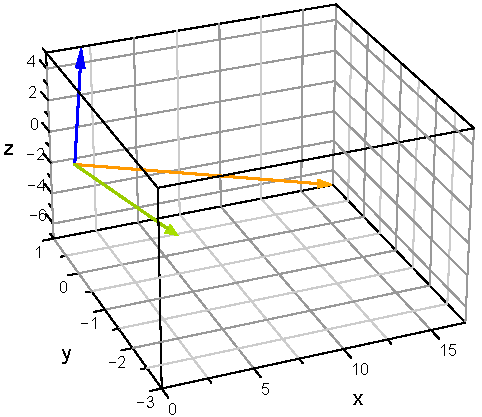
\includegraphics[width=0.5\linewidth]{mai_fig025.pdf}
    \captionof{figure}[Ortogonální doplněk]{Vizualizace vektorového prostoru a jeho    
             ortogonálního doplňku pomocí sw MatLab - MuPAD příkazem:\newline
             \texttt{plot(plot::Arrow3d([1,-3,2]), plot::Arrow3d([2,1,5]), 
             plot::Arrow3d([17,1,-7]))}}
    \label{LA:fig_ort01}
    \par}
\end{example}

      %---------------------------------------------------------------
  
      Výsledek předchozího příkladu \ref{mai:exam011} lze interpretovat tak, že jsme našli všechny 
      vektory, které jsou kolmé na rovinu určenou vektory ze zadání. Rovina je útvar       
      dvojrozměrný a protože prostor všech vektorů je trojrozměrný, musí nutně mít podprostor 
      ortogonálních vektorů ve shodě se vztahem \ref{LA:eq_dim_doplnek} pouze jednu dimenzi. Vše 
      je dobře patrné z obr. \ref{LA:fig_ort01}

%} % tikzset
%---------------------------------------------------------------------------------------------------
%\printbibliography[title={Seznam literatury}, heading=subbibliography]
\addcontentsline{toc}{section}{Seznam literatury}
              